\documentclass[../../main/main.tex]{subfiles}
\begin{document}

\section{Monotone and Continuous Strategy Proofs}
\label{app:monotone_proofs}

This appendix provides the detailed proofs regarding monotone calling strategies, monotone-admissible and continuous betting strategies, and their relationship to the uniqueness of the Nash equilibrium in LCP.

\subsection{Monotone Strategies and Weak Dominance}

\begin{lemma}
    \label{lem:monotone_dominated}
    If a calling strategy violates the first monotonicity condition (see \ref{subsec:monotone_strategies}) for a nonzero-measure set of hands for any bet size $s$, it is weakly dominated. Specifically, if there exists $s$ and measurable sets $A, B \subseteq [0, 1]$ such that:
    \begin{enumerate}
        \item The caller calls $s$ with hands in $A$
        \item The caller folds $s$ with hands in $B$
        \item $\sup A \leq \inf B$
        \item $A$ and $B$ have positive measure
    \end{enumerate}
    then the strategy is weakly dominated.
\end{lemma}

\begin{proof}
    Let $\sigma_C$ be the non-monotone strategy described above. Since $A$ and $B$ are nonzero-measure, there exist subsets $A' \subseteq A$ and $B' \subseteq B$ such that:
    \begin{enumerate}
        \item $A'$ and $B'$ have positive measure
        \item $|A'| = |B'|$
    \end{enumerate}
    Where $|A|$ and $|B|$ denote the Lebesgue measure of $A$ and $B$ (see Figure \ref{fig:strategy_improvement}).

    \begin{figure}[h]
        \centering
        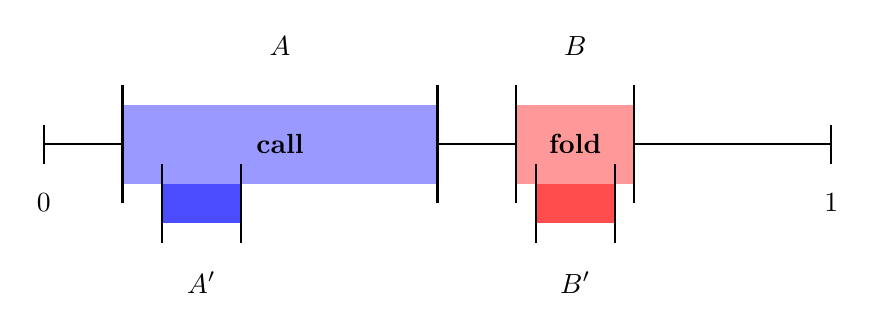
\begin{tikzpicture}[scale=5]
            % Number line from 0 to 1
            \draw[thick] (0,0) -- (2,0);

            % Tick marks at 0 and 1
            \draw[thick] (0, -0.05) -- (0, 0.05);
            \draw[thick] (2, -0.05) -- (2, 0.05);

            % Endpoint labels
            \node[below] at (0, -0.1) {$0$};
            \node[below] at (2, -0.1) {$1$};

            % Set A (calling hands) - blue
            \fill[blue!40] (0.2, -0.1) rectangle (1.0, 0.1);
            \draw[thick] (0.2, -0.15) -- (0.2, 0.15);
            \draw[thick] (1.0, -0.15) -- (1.0, 0.15);
            \node[above] at (0.6, 0.2) {$A$};
            \node at (0.6, 0) {\textbf{call}};

            % Set B (folding hands) - red
            \fill[red!40] (1.2, -0.1) rectangle (1.5, 0.1);
            \draw[thick] (1.2, -0.15) -- (1.2, 0.15);
            \draw[thick] (1.5, -0.15) -- (1.5, 0.15);
            \node[above] at (1.35, 0.2) {$B$};
            \node at (1.35, 0) {\textbf{fold}};

            % Set A' (subset of A) - darker blue
            \fill[blue!70] (0.3, -0.2) rectangle (0.5, -0.1);
            \draw[thick] (0.3, -0.25) -- (0.3, -0.05);
            \draw[thick] (0.5, -0.25) -- (0.5, -0.05);
            \node[below] at (0.4, -0.3) {$A'$};

            % Set B' (subset of B) - darker red
            \fill[red!70] (1.25, -0.2) rectangle (1.45, -0.1);
            \draw[thick] (1.25, -0.25) -- (1.25, -0.05);
            \draw[thick] (1.45, -0.25) -- (1.45, -0.05);
            \node[below] at (1.35, -0.3) {$B'$};

        \end{tikzpicture}
        \caption{A simple case of sets $A$ and $B$ which violate monotonicity ($\sup A \leq \inf B$). We can find equal-measure subsets $A' \subseteq A$ and $B' \subseteq B$ to swap actions, improving the strategy.}
        \label{fig:strategy_improvement}
    \end{figure}

    The existence of such subsets follows from a fundamental property of nonatomic measures: since the uniform distribution on $[0,1]$ is nonatomic (no single point has positive probability), for any two measurable sets with positive measure, we can always find measurable subsets of equal measure\cite{Sierpinski1922}. This property allows us to construct the strategy improvement described below.

    Let $\sigma_C'$ be the strategy which switches the actions for $A'$ and $B'$, i.e. calls with $B'$ and folds with $A'$ (and behaves identically for all other bet sizes). We now analyze how this change affects the caller's performance against any betting strategy.

    Against a bet of size $s$, the key improvement occurs in two scenarios:
    \begin{enumerate}
        \item When $y \in B'$ and $x \in A'$: $\sigma_C$ folds while $\sigma_C'$ calls and wins (since $x \in A$ and $y \in B$ with $\sup A \leq \inf B$)
        \item When $y \in A'$ and $x \in B'$: $\sigma_C$ calls and loses while $\sigma_C'$ folds (avoiding the loss)
    \end{enumerate}

    For all other cases, $\sigma_C$ and $\sigma_C'$ behave identically, so $\sigma_C'$ is weakly better than $\sigma_C$ against every betting strategy.

    To show that $\sigma_C$ is strictly dominated, consider a betting strategy which always bets $s$. Against this strategy, both scenarios above occur with positive probability (since $A'$ and $B'$ have positive measure), so $\sigma_C'$ is strictly better than $\sigma_C$. Thus, $\sigma_C$ is weakly dominated.
\end{proof}

We now show that the restriction to monotone-admissible betting strategies implies a natural ordering of bluff sizes.

\begin{lemma}
\label{lem:bluff_monotonicity}
If a betting strategy $\sigma_B$ is monotone-admissible, then for any two bluffing hands $x < x'$ with corresponding bet sizes $s$ and $s'$ respectively, we must have $s' \geq s$.
\end{lemma}

\begin{proof}
Suppose for contradiction that there exist bluffing hands $x < x'$ with bet sizes $s > s'$. We will show that $\sigma_B$ is not monotone-admissible by constructing a strategy $\sigma_B'$ that weakly dominates $\sigma_B$ against all monotone calling strategies.

Define $\sigma_B'$ to be identical to $\sigma_B$ except that it bets $s'$ with hand $x$ instead of $s$.

Let $\sigma_C$ be an arbitrary monotone calling strategy, and let $c(s)$ denote the calling threshold for bet size $s$ under $\sigma_C$. By Definition~\ref{def:monotone_calling} (condition 2), monotonicity implies
\[
c(s') \leq c(s).
\]

We compare the expected payoffs of betting $s$ versus $s'$ with hand $x$ against $\sigma_C$.

\textbf{Case 1:} $x' < c(s')$.

Since $c(s') \leq c(s)$, we have $x < x' < c(s') \leq c(s)$. Thus the caller never calls with a hand weaker than $x$ or $x'$ under either bet size. Both bets succeed as pure bluffs with probability $P(Y < c(\cdot))$, winning the pot of size $1$. Since $s' < s$, betting $s'$ risks less to win the same amount, so
\[
\mathbb{E}[\text{payoff of } s' \mid x] > \mathbb{E}[\text{payoff of } s \mid x].
\]

\textbf{Case 2:} $x' \geq c(s')$.

When betting $s'$ with hand $x$, the bettor wins at showdown against any caller hand $y \in [c(s'), x']$, an event with positive probability. When betting $s$ with hand $x$, since $c(s) \geq c(s') > x$, the bettor never wins at showdown (as $x < c(s)$ implies all calling hands beat $x$). Therefore,
\[
\mathbb{E}[\text{payoff of } s' \mid x] > \mathbb{E}[\text{payoff of } s \mid x].
\]

In both cases, $\sigma_B'$ achieves strictly higher expected payoff than $\sigma_B$ against $\sigma_C$. Since this holds for all monotone calling strategies $\sigma_C$, strategy $\sigma_B$ is not monotone-admissible, contradicting our assumption.
\end{proof}


\subsection{Continuity}

We stated in section \ref{sec:solving_lcp} that the betting strategy should be continuous except at the bluffing and value-betting thresholds.
Here we provide a formal justification for this requirement.

Consider the bettor's expected value function for a value hand $x$:
\begin{equation}
    EV(s, x) = (x - c(s))(1 + s) - (1 - x)s + c(s)
\end{equation}

which is continuous in both $s$ and $x$. For a fixed value-betting hand strength $x$, the bettor chooses an optimal bet size $s^*(x)$ such that:

\begin{equation}
    s^*(x) = \arg\max_{s \in [L, U]} EV(s, x)
\end{equation}

Assuming $EV(s, x)$ is strictly concave in $s$ (which follows if $c(s)$ is sufficiently smooth and monotone increasing), the maximizer $s^*(x)$ is unique. By the Theorem of the Maximum \cite{stokey1989recursive}, since $EV(s, x)$ is continuous and the set of possible bet sizes $S$ is compact, the optimal strategy $s^*(x)$ is a continuous function of $x$. 

If $s(x)$ were discontinuous at some $x_0$, it would imply that $EV(s, x)$ possesses multiple global maxima at $x_0$, or that the $EV$ function itself is not concave, allowing the optimal bet size to ``jump" between distant peaks.

For the bluffing range, continuity is a consequence of the equilibrium balancing requirement. To maintain the caller's indifference at every $s \in [L, U]$, there must exist a corresponding bluffing hand strength such that the ratio of bluffs to value hands satisfies the Nash condition.

As previously established, the bluffing strategy $b^{-1}(x)$ is strictly decreasing in $x$ as a consequence of being monotone-admissible. Since every $s \in [L, U]$ must be represented in the bluffing range to balance the value bets, the image of $b^{-1}(x)$ is the interval $[L, U]$. 

By the Intermediate Value Theorem for Monotone Functions (the property that a monotonic function is continuous if and only if its image is an interval), $b^{-1}(x)$ must be continuous.

\end{document}
